\documentclass{article}
\usepackage[utf8]{inputenc}
\usepackage[T1]{fontenc}
\usepackage[font=footnotesize]{caption}
\usepackage{fancyhdr}
\usepackage[document]{ragged2e}
\usepackage[super]{nth}
\usepackage{parskip}
\usepackage{hyperref}
\usepackage{capt-of}
\usepackage{graphicx}
\graphicspath{ {./} }
\pagestyle{headings}
\setlength{\parindent}{0pt}

\textwidth = 460pt
\oddsidemargin = 10pt
\topmargin = -60pt
\textheight = 690pt

\title{\textbf{Analysis of Voice Data towards Biometric Identification:\\ Gender, Age and Identity Classification}\par Computer-Aided Diagnostics}
\author{
João Carlos Ramos Gonçalves de Matos – up201704111\\
Maria Jorge Miranda Loureiro – up201704188\\
Maria Manuel Domingos Carvalho – up201706990\\
}
\date{\nth{15} January 2021}

\begin{document}

\maketitle
\thispagestyle{empty} 

\justify
\normalsize
\setlength{\parindent}{0pt}

\textbf{\emph{Abstract - Add abstract} }
\vspace{2mm}

Cenas a reter da reunião para o relatório:\par
- Tentar o melhor modelo para certo objetivo, reportando os restantes\par
- conclusões extra: se os melhores modelos forem não lineares podemos então dizer que o problema deve ser linear\par
- Subject dependent/independent - testar os dois e explicar as suas possíveis aplicações em cada situação: dependent pode ser usado para personalizar o modelo em pessoas especificas\par
- Comparar resultados com state of the art, se for 5/10\% abaixo do artigo, ta top.\par


\textbf{\emph{Keywords - Add keywords (maybe 4/5) } }
\vspace{2mm}

\textbf{I. Introduction}\par

\vspace{2mm}
\textbf{II. Data Preparation }\par

\vspace{2mm}
\textbf{ A. Feature Extraction }\par
To train machine learning models to classify gender, age and identity, voice signal features can be used as the training set of these models. Taking into account the different features considered relevant in the literature [1,2] , a set of signal features were chosen and extracted from all the utterances in the database (Table 1). The pyAudioAnalysis (version 0.3.6) python library was used to extract all audio features.

At first, each model was trained with the complete set of features. Then, to reduce the dimension of the dataset, remove redundant information and reduce running cost, Principal Component Analysis was applied, downsizing the number of features from 136 to 35, by setting the desired explained variance to 99\% \textbf{(alterar se mudarmos este parâmetro!!) } [3,4].

\begin{center}
\captionof{table}{List of all features extracted from voice signals.}
\label{table1} % for use in \ref{table1} - to refer to the table number
\begin{tabular}[c]{ |c| } 
 \hline
 \textbf{Feature Name}  \\ [1ex]
 \hline
 Zero Crossing Rate \\ [0.5ex]
 Energy \\ [0.5ex]
 Entropy of Energy \\ [0.5ex]
 Spectral Centroid  \\ [0.5ex]
 Spectral Spread \\ [0.5ex]
 Spectral Entropy \\ [0.5ex]
 Spectral Flux \\ [0.5ex]
 Spectral Rolloff \\ [0.5ex]
 12 Mel Frequency Cepstral Coefficients \\ [0.5ex]
 11 Chroma Vectors \\ [0.5ex]
 Chroma Deviation \\ [0.5ex]
 \hline
\end{tabular}
\end{center}

\vspace{2mm}
\textbf{ B. Feature Selection }\par

- Explicar anova se efetivamente usarmos!\par

\vspace{2mm}
\textbf{ C. Dataset Split }\par
- Explain the 10 nested hold outs and why we did that.
- why we separated native vs English utterances.\par

\vspace{2mm}
\textbf{ D. Defining Classification Groups }\par
- Explain how we divided age - se usarmos regressão e cagarmos nos grupos acho que podemos tirar isto!\par



\vspace{2mm}
\textbf{III. Experiments, Results and Discussion }\par

\vspace{2mm}
\textbf{ A. Gender Classification }\par

- Explain Method Logistic Regression
- Explain Method Random Forest (livro pag. 333)
- Explain Method SVM
- Explain Method MLP Classifier (livro cap. 18)
- Show results of all of them (maybe a proper table? maybe even join english vs native in one big table to save space)
- Analyse results (including native vs english)

\vspace{2mm}
\textbf{ B. Age Classification }\par

- Explain different approaches
- Show results of all of them (maybe a proper table? maybe even join english vs native in one big table to save space)
- Analyse results (including native vs english)

\vspace{2mm}
\textbf{ C. Open and Closed World Identity Classification }\par
Towards the identification of specific subjects in a subset of voice utterances, a pipeline to perform open-world and closed-world classification was designed. Figure \ref{fig:identificationScheme} illustrates the representative scheme of this approach.\par

Gaussian Naive Bayes was used to model each identity class, present in the subjects database, and it employees a diagonal co-variance matrix to each model, assuming features independence. After the creation of the database, with both english and native utterances for each subject, the audio track in analysis was tested in each model and the probability of the sample belonging to each class was computed. When the probability of belonging to the positive class, which is indeed modeling a specific identity, is equal to 1, the track is considered identified.\par

- Explicar testes feitos e resultados obtidos!!\par

\begin{figure}
\caption{Scheme of the Open and Closed-World Classification Pipeline.}
\centering
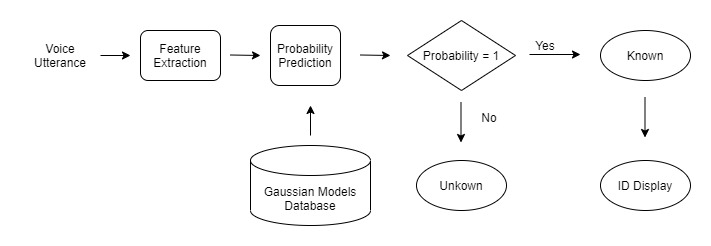
\includegraphics[scale=0.4]{DACOIdentities.jpg}
 \label{fig:identificationScheme}
\end{figure}

\vspace{2mm}
\textbf{IV. Conclusions }\par


\vspace{2mm}
\textbf{V. References}\par
[1]	O. Iloanusi et al., Voice Recognition and Gender Classification in the Context of Native Languages and Lingua Franca. 2019, pp. 175-179.\par
[2] Rami S. Alkhawaldeh, "DGR: Gender Recognition of Human Speech Using One-Dimensional Conventional Neural Network", Scientific Programming, vol. 2019, 12 pages, 2019.
[3] https://www.mikulskibartosz.name/pca-how-to-choose-the-number-of-components/
[4] https://medium.com/datadriveninvestor/principal-component-analysis-pca-a0c5715bc9a2
\end{document}